\documentclass[12pt,a4paper,notitlepage]{article}
\linespread{2.0}

\usepackage[T1]{fontenc}
\usepackage[utf8]{inputenc}
\usepackage{hyperref}
\usepackage{mathtools}
\usepackage{graphicx}

\begin{document}

\title{Technical Report on Convolutional Neural Networks}
\author{Sebastien Champoux 40133449
\\ ENGR 411 Technical Report
\\ Concordia University - Department of Computer Science
\\ Winter 2022
\\ Presented to Professor Nematollaah Shiri
}
\maketitle

\begin{abstract}
Convolutional neural networks are a class of artificial neural networks that are commonly used to analyze digital imagery. This report will discuss the functioning of CNNs in the context of image classification.
\end{abstract}
\clearpage

\tableofcontents
\clearpage

\listoffigures
\clearpage

\section{Introduction}
Neural networks are one amongst many forms of machine learning that were developed in the last decades. Convolutional neural networks are a specialized form of neural networks that are especially well suited for image analysis, such as identifying and classifying objects within images. The following report will discuss different aspects of convolutional neural networks  in the specific context of image classification: their structures, the deep learning process, image convolutions, pooling, and a discussion of favorable characteristics that make CNNs well-suited for image analysis.

\section{Fully-connected neural networks}\label{fully-connected-networks}
In order to perform image classification, convolutional neural networks process images by image convolutions, before feeding the processed data into a fully-connected neural network, also known as a multilayer perceptron. This section will cover this latter step, the fully connected neural network. The other layers of CNNs over multilayer perceptrons will be discussed in section \ref{cnn-section}.

\subsection{Structure}
A classical concrete application of a neural network is the identification of handwritten digits. This application is commonly used as an example thanks to the existence of the MNIST Database (\textit{Modified National Institute of Standards and Technology database}), a database of 70,000 labelled pictures of handwritten digits freely available for machine learning \cite{lecun_mnist_1998}. To simplify the presentation of multilayer perceptrons below, this application will be used to illustrate how the different components of a neural network can work together to achieve this application.

A multilayer perceptron is a class of neural network. As the name implies, it is made up of "neurons" that are connected together. A neuron is simply a real number in the range [0,1] that represents an activation; 0.0 meaning the neuron is not activated and 1.0 meaning the neuron is fully activated. The neurons are arranged in multiple layers, at least three: an input layer, an output layer, and at least one "hidden" layer, each one serving a different role.

The neurons in the input layer represent a part of the total input provided to the neural network. For the digits example, the input is a black and white image of a handwritten digit, of dimensions 28*28 pixels. Therefore, the input layer would contain 784 neurons, each corresponding to a pixel of the image, and their respective activation being the brightness value of their respective pixel (0.0 being black, 1.0 being white, and shades of grey in-between) \cite{sanderson_but_2017}.

The output layer represents the output of the neural network. As the perceptron performs recognition and classification, each neuron in the output layer is one of the possible "choices" of what could be represented in the image. For the digits example, the output layer would contain ten neurons, one for each digit. The intended output of the neural network is for all but one of the output neurons to have a low activation, and one neuron having a very high activation, the latter being the network's best guess of what digit is represented in the image.

The hidden layers, in-between the input and output layers, serve to improve the performance of the neural network. These layers enable the network to recognize patterns within the image, therefore facilitating the recognition of complex forms. For instance, the digit "8" is made up of two small loops one over the other. In theory, the middle layers could attempt to recognize these shapes in the image to make a decision whether the digit represented is an eight. In practice, neural networks create their own patterns during the training process, which are often very abstract and a far cry of what a human would consider logical \cite{sanderson_gradient_2017}.

In a standard multilayer perceptron, every neuron from a layer is connected to every neuron from the previous layer. The activation of a neuron impacts the activation of every neuron connected to it. In other words, with the exception of the input layer, neurons are functions of the activation of the neurons that preceed them. The connection in-between two layers can be weighted, to increase or decrease how much the activation of a neuron impacts the connection of another neuron.

\begin{figure}[htbp]
	\centering
		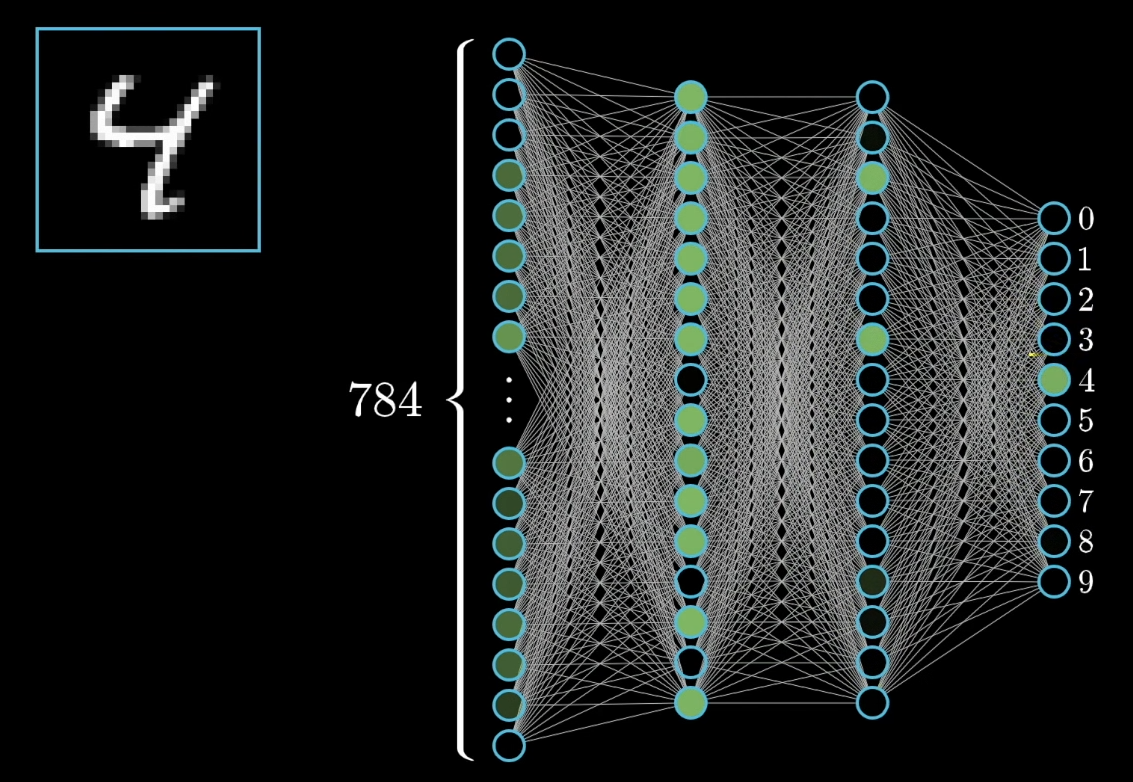
\includegraphics[width=0.60\textwidth]{images/perceptron-visualisation.png}
	\caption{Visualisation of a multilayer perceptron \cite{sanderson_gradient_2017}}
	\label{fig:perceptron-visualisation}
\end{figure}

A bias can also be introduced into the equation. The addition of a bias can help improve the results by requiring a very high, or very low, activation in parts of the input to activate some neurons in the following layers \cite{sanderson_but_2017}.

All of these elements can be summarized into a vector-matrix multiplication. Below is the equation to compute the activation of the neurons in hidden layer 1, based on the activation of neurons from the input layer (layer 0). \(a_i^{(0)}\) represents the activation of neuron \(i\) from layer 0, \(w_{i,j}\) the weight of the connection between neuron \(i\) from the input layer and neuron \(j\) in layer 1, and \(b_i\) the bias applied to the weighted sum of the incoming connections from all of layer 0 to neuron \(i\) in layer 1. This output vector is processed through a function, usually the sigmoid function, to squish the results into the range \([0,1]\). This output neuron represents the activation of every neuron in layer 1. This process can then be repeated for the subsequent layers, using the activation vector of layer 1 as input \cite{sanderson_but_2017}.

\begin{displaymath}
	\sigma
	\left(
	\begin{bmatrix}
		w_{0,0} & w_{0,1} & \cdots & w_{0,n}\\
		w_{1,0} & w_{1,1} & \cdots & w_{1,n}\\
		\vdots & \vdots & \ddots & \vdots\\
		w_{m,0} & w_{m,1} & \cdots & w_{m,n}
	\end{bmatrix}
	\begin{bmatrix}
		a_{0}^{(0)}\\
		a_{1}^{(0)}\\
		\vdots\\
		a_{n}^{(0)}
	\end{bmatrix}
	+
	\begin{bmatrix}
		b_{0}\\
		b_{1}\\
		\vdots\\
		b_{n}
	\end{bmatrix}
	\right)
	=
	\begin{bmatrix}
		a_{0}^{(1)}\\
		a_{1}^{(1)}\\
		\vdots\\
		a_{n}^{(1)}
	\end{bmatrix}
\end{displaymath}

As demonstrated above, a neural network boils down to a linear algebraic function. For this reason, neural networks are often computed by graphical processing units (GPUs) instead of regular CPUs, as they are optimized for processing vector-matrices computations \cite{salter_cart_2021}.

\subsection{Deep learning, gradient descent and backpropagation}\label{deep-learning}
\subsubsection{Description of the process}
Once the structure of the neural network has been laid down, it must be tuned so that it can recognize and classify accurately what is presented to it. This tuning process consists of adjusting the hundreds of weights and biases that connect the neurons, such that the neural network returns acceptable results over a large training set. Given the numerous weights and biases, this is too tedious and intricate to be performed by humans. Therefore, the neural network "trains itself" with the help of two algorithms, gradient descent and backpropagation. \cite{ibm_cloud_education_what_2020}.

To train a neural network, it is necessary to have a training set on-hand. A training set is a set of content (images, videos, audio clips or some other medium), in which each item is labelled with the expected classification. As discussed earlier, the MNIST database is a good example of a training set: it is a set of 70,000 images of hand-drawn digits, each image appropriately labelled with the represented digit \cite{lecun_mnist_1998}. Another example is the database created by Google's ReCAPTCHA service. This service helps to protect websites from bots by asking users to identify objects within images. By doing so, human users of ReCAPTCHA are also, unknowingly, contributing to the elaboration of training sets for AI training \cite{maruzani_are_2021}.

To begin the training process, the different weights and biases of the neural network are initialized with random values. Then, the training set is processed by the neural network. After this first test, the results will be very poor. The network computes the accuracy (or lack thereof) of its results with a cost function. This function receives, as input, the different weights and biases in the neural network, and returns a real number, the average cost of the network's errors over the training set.

Below is the cost function of the neural network for one element of the training set. It is the sum of the squared difference between the activation of each neuron in the output layer (\(a_{j}^{(L)}\)) and their expected activation (\(y_{j}^{(L)}\)).
\begin{displaymath}
	C_{0} = \sum_{j=0}^{n_{L} - 1} (a_{j}^{(L)} - y_{j})^{2}
\end{displaymath}
This cost function expresses how accurate the results given by the neural network are. The higher the error cost, the greater the difference between the expected and computed results and thus, the less accurate the network. The objective is to adjust the weights and biases in the neural network to decrease this error cost as close as possible to 0 for the training set.

To reduce this cost function, gradient descent will be used. Gradient descent is an optimization algorithm to find a local minimum of a function. It consists of computing the gradient of the cost function (noted \(\nabla C\) - a vector in the direction of the steepest increase for each weight and bias of the network), adjusting the weights and biases by a factor of the negative of this vector (\(-\nabla C\)), and repeating these steps until a local minimum is reached \cite{sanderson_gradient_2017}.

The algorithm to efficiently compute the gradient of a neural network is backpropagation. This algorithm computes the gradient vector that is used to minimize the error cost. For each element in the training set, the algorithm starts from the output layer, and compares the activation of the output layer's neurons to the expected result. Then, it computes by how much each weight and bias that connect the output layer to its previous layer should be adjusted in order to minimize the error cost (in other words, decrease the difference between the output neurons' actual and expected activation). Connections (weights) that improve the accuracy of the results should be strengthened, and inversely, connections that worsens the results should see their weight diminished. Furthermore, these adjustments should be proportional to how much each connection impacts the error cost. This procedure is repeated recursively for each layer, from the output to the input layer. Finally, the adjustments computed for each example in the training set are averaged to get an adjustment vector for the entire training set. This algorithm is repeated multiple times until an acceptable accuracy is reached \cite{sanderson_gradient_2017}.

Computing the error cost and gradient descent of a neural network over a training set of tens of thousands of examples is computationally expensive. For this reason, a more performant technique, stochastic gradient descent, is commonly used. The algorithm is the same, but instead of computing the entire training set, the training set is subdivided into multiple smaller random subsets of training examples. Then, the gradient descent vector is computed for every subset of the training set, and these vectors are applied iteratively to gradually improve the results of the network \cite{sanderson_gradient_2017}.


\subsubsection{Calculus of deep learning}
The process described above is achieved by the use of derivatives and the chain rule of calculus.

The equation below is the weighted sum of the activation of the neurons of the previous layer, plus a bias. In other words, it is the activation of a neuron that has not yet been processed through the sigmoid function. Note that this weighted sum is represented as \(z_j^{(L)}\) to differentiate it from the activation of a neuron (represented as \(a_j^{(L)}\) in the second equation below). This equation is presented here separately from the activation function because it will be used to compute the cost function's gradient.
\begin{displaymath}
	z_j^{(L)} = w_{j0}^{(L)}a_0^{(L-1)} + w_{j1}^{(L)}a_1^{(L-1)} + \cdots + w_{jk}^{(L)}a_k^{(L-1)} + b_j^{(L)}
\end{displaymath}

Thus, the activation for a neuron in the neural network can be represented as:
\begin{displaymath}
	a_j^{(L)} = \sigma\left(z_j^{(L)}\right)
\end{displaymath}

The derivative of the cost function over the derivative of a specific weight is necessary for this computation. It is represented in the equation below. Not all connections in the network have an equal impact on the error cost ; this equation tells us how much a specific weight or bias in the neural network impacts the error cost.
\begin{displaymath}
	\frac{\delta C_0}{\delta w_{jk}^{(L)}} = a^{(L-1)} \sigma\prime(x^{(L)})((a^{(L)})^2)\prime
\end{displaymath}

Below: derivative of cost function in relation to a specific activation. Tells how sensitive cost is to a specific activation in the previous layer (L-1). Neuron influences cost through multiple different "paths" which is why we sum those influences together.
\begin{displaymath}
	\frac{\delta C_0}{\delta a_{k}^{(L-1)}} = 
	\sum_{j=0}^{n_{L-1}}
	\frac{\delta z_j^{(L)}}{\delta a_{k}^{(L-1)}}
	\frac{\delta a_j^{(L)}}{\delta z_j^{(L)}}
	\frac{\delta C_0}{\delta a_j^{(L)}}
\end{displaymath}

Therefore, by using the chain rule, it is possible to compute the derivative of the cost function in relation to a specific weight. This equation tells us how much an adjustment to this weight will impact the error cost.
\begin{displaymath}
	\frac{\delta C_0}{\delta w_{jk}^{(L)}} = 
	\frac{\delta z_j^{(L)}}{\delta w_{jk}^{(L)}}
	\frac{\delta a_j^{(L)}}{\delta z_j^{(L)}}
	\frac{\delta C_0}{\delta a_j^{(L)}}
\end{displaymath}

The result is the gradient descent vector. Each component of this vector represents the adjustments that should be made to the different weights and biases in the neural network to minimize the cost function.
\begin{displaymath}
	-\nabla C =
	-1 \begin{bmatrix}
		\frac{\delta C_0}{\delta w_{0,0}^{(1)}}\\
		\frac{\delta C_0}{\delta w_{0,1}^{(1)}}\\
		\vdots\\
		\frac{\delta C_0}{\delta w_{j,k}^{(1)}}\\
		\frac{\delta C_0}{\delta b_{0}^{(1)}}\\
		\vdots\\
		\frac{\delta C_0}{\delta b_{k}^{(1)}}\\
	\end{bmatrix}
\end{displaymath}

\section{Convolutional and pooling layers}
Convolutional neural networks are enhanced multilayer perceptrons that feature at least two additional, special purpose layers: a convolutional layer and a pooling layer. The image data is first processed through these two layers, and is subsequently flattened into an array to be fed to a regular perceptron for the purpose of classification, as discussed in section \ref{fully-connected-networks} \cite{saha_comprehensive_2018}.

\begin{figure}[htbp]
	\centering
		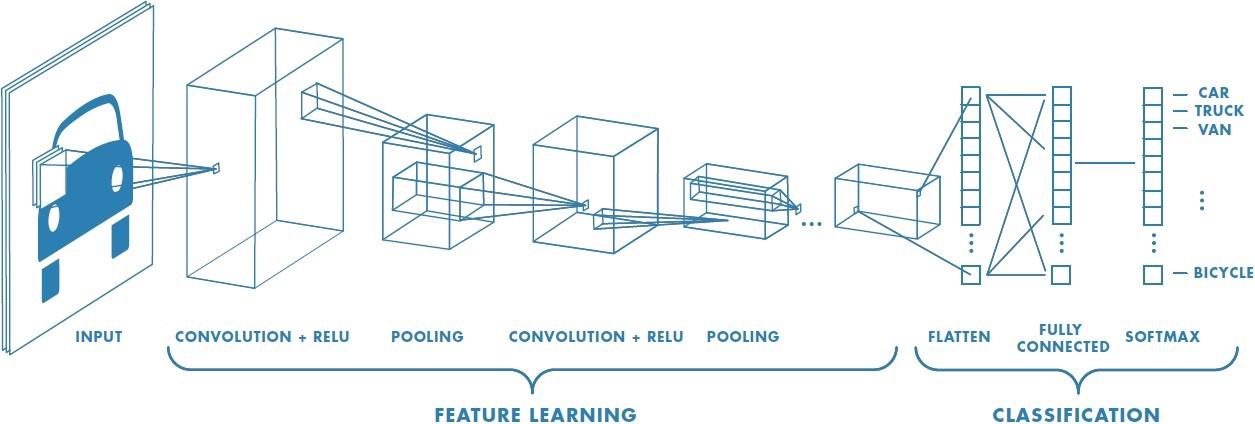
\includegraphics[width=0.70\textwidth]{images/convolutional-neural-network.jpeg}
	\caption{Illustration of a convolutional neural network \cite{saha_comprehensive_2018}.}
	\label{fig:convolutional-neural-network}
\end{figure}

\subsection{Image convolutions}
Image convolutions is a technique of image processing to create different renditions of images, such as blurring, sharpening, highlighting edges, etc. It consists of applying a kernel, i.e., a small matrix, over the image, by image convolutions. An image convolution consists of computing the weighted average of the values of each group of pixel of the same size as the kernel, according to the pixel weights defined in the kernel \cite{sanderson_convolutions_2020}.

\begin{displaymath}
	\begin{bmatrix}
		1/9 & 1/9 & 1/9 \\
		1/9 & 1/9 & 1/9 \\
		1/9 & 1/9 & 1/9
	\end{bmatrix}
\end{displaymath}

\begin{figure}[htbp]
	\centering
		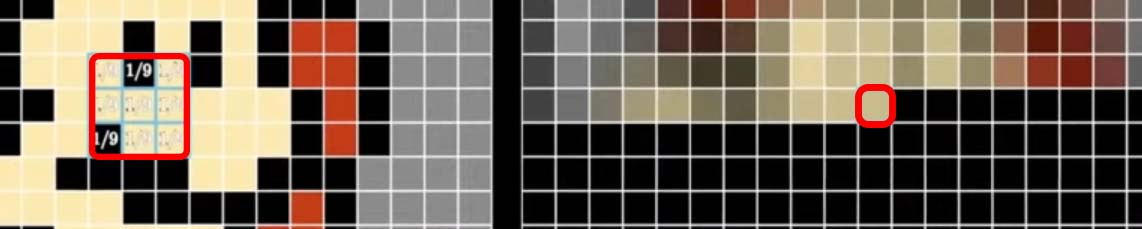
\includegraphics[width=1.00\textwidth]{images/box-blur.jpg}
	\caption{A group of beige and black pixels are averaged to a grey-beige by the box blur kernel \cite{sanderson_convolutions_2020}.}
	\label{fig:box-blur}
\end{figure}

As a simple example, the kernel above would create a box blur effect. For each group of 9 pixels in the original image, the corresponding center pixel in the blurred image would be equal to an average of the 9 pixels, all with equal weights.

Another example of a possible simple kernel is \(\begin{bsmallmatrix}-1 & -1 & -1 \\ 1 & 1 & 1 \\ 0 & 0 & 0\end{bsmallmatrix}\). This kernel would highlight top edges of objects in an image \cite{deep_lizard_convolutional_2017}.

\begin{figure}[htbp]
	\centering
		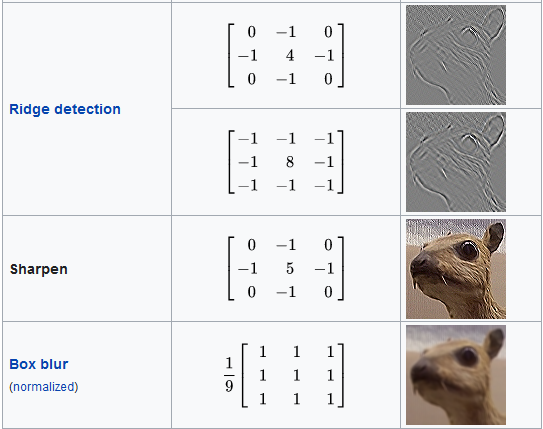
\includegraphics[width=0.8\textwidth]{images/image-convolutions-examples.png}
	\caption{Examples of kernels and their application on a sample image \cite{wikipedia_collaborators_kernel_2022}}
	\label{fig:image-convolutions-examples}
\end{figure}

An issue arises when the kernel is applied to pixels close to the edges. As each kernel of n * n pixels renders a single pixel in the image convolution, there will be a discrepancy between the original and convoluted image when the kernel is applied near the edges. Two techniques are used to deal with this situation: \textbf{valid padding} and \textbf{solid padding}. For valid padding, the original image is padded with additional blank pixels beyond the edges, such that the convoluted image has the same dimensions as the original image. For same padding, the original image is not padded, and the kernel is applied up to the image's edges only. This results in a convoluted image that is a few pixels smaller than its original \cite{sanderson_convolutions_2020}.

\begin{figure}[htbp]
	\centering
		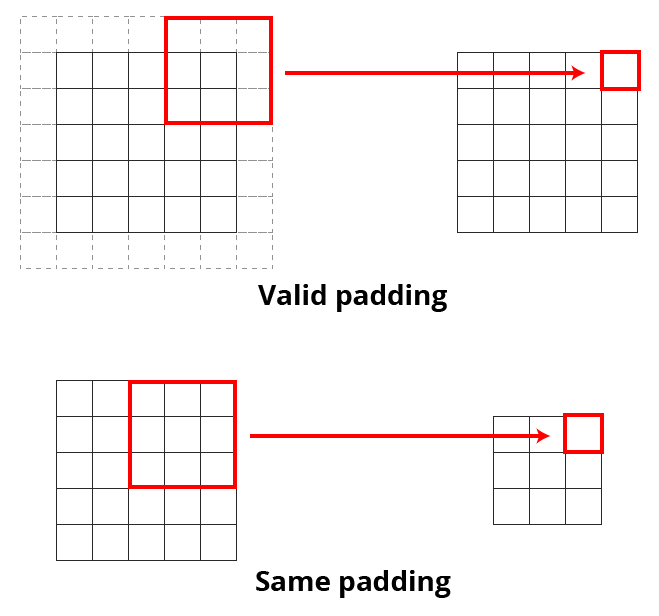
\includegraphics[width=0.80\textwidth]{images/padding-illustration.png}
	\caption{Comparison of same and valid padding algorithms}
	\label{fig:padding-illustration}
\end{figure}

\subsection{Convolutional layers}\label{cnn-section}
The convolutional layers apply image convolutions with different kernels to the input images in order to extract additional information from them. The objective of the convolution operation is to extract high-level features from the input image, such as edges or corners. If multiple convolutional layers are used, conventionaly, the additional layers will be responsible for detecting higher-level features, such as shapes or patterns. With enough layers, a convolutional neural network can acquire some very deep insight into the subject of the image \cite{saha_comprehensive_2018}.

[À adapter] In the case of images with multiple channels (e.g. RGB), the Kernel has the same depth as that of the input image. Matrix Multiplication is performed between Kn and In stack ([K1, I1]; [K2, I2]; [K3, I3]) and all the results are summed with the bias to give us a squashed one-depth channel Convoluted Feature Output.

The kernels used in the convolutional layers can be specified by hand. However, they can also be learned using the technique described in section \ref{deep-learning}, which is a strength of convolutional neural networks \cite{brownlee_gentle_2019}.

\subsection{Pooling layers}
The convolutional layers are very effective at highlighting features within an image, but they also have the downside of recording their precise location within the image frame. Therefore, transformations to the image, such as cropping, rotating or shifting will alter the feature map \cite{brownlee_gentle_2019}.

The most common approach to this problem is downsampling. Downsampling reduces the dimensions and resolution of the image. This results in a less detailed feature map, that preserves the large, important details, while foregoing the minor, less useful ones. This also diminishes the impact that the position, rotation or scale of an object has on the neural network's output. One technique to downsampling is to change the stride of the image convolution. This simply means that when a kernel is convoluted over an image, instead of applying the kernel to every pixel, the kernel is only applied to every \(n^{th}\) pixel. This technique can work, but a more robust approach is to use a pooling layer.

A pooling operation is applied to every feature map produced by the convolution layers. For every group of n * n pixels in an image, a math operation is applied to create a single value. The size of the pooling operation is almost always 2*2, which means that every image dimension will be reduced by half, and the number of pixels will be reduced by a factor of four \cite{brownlee_gentle_2019}.

There are two common pooling algorithms: \textbf{max pooling} and \textbf{average pooling}. Max pooling returns the maximum value from each kernel of n * n pixels. Average pooling returns the average of the \(n^2\) pixels' values within a kernel. Max pooling is generally preferred because, in addition to reducing the image's dimension, it also discards unusual, noisy activations from the data, whereas average pooling does not discard noise \cite{saha_comprehensive_2018}.

Unlike convolutional layers, pooling layers are not machine-learned. They are always specified by the programmmer \cite{brownlee_gentle_2019}.

\begin{figure}[htbp]
	\centering
		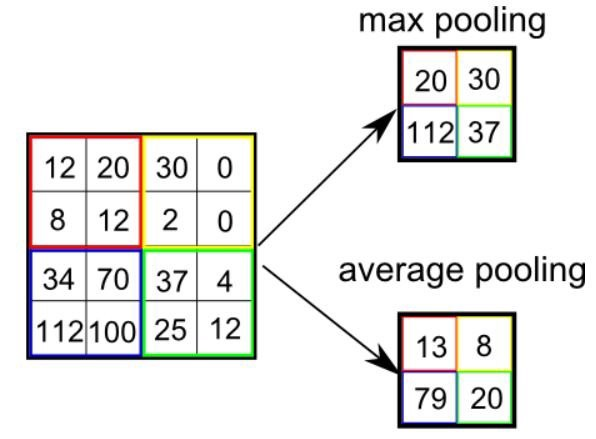
\includegraphics[width=0.80\textwidth]{images/pooling.jpg}
	\caption{Comparison of max and average pooling algorithms \cite{saha_comprehensive_2018}}
	\label{fig:pooling}
\end{figure}

\subsection{Image classification}
After processing the image through the convolutional and pooling layers, the remaining data is flattened into an array of numbers. This array is fed into a multilayer perceptron, as discussed in section \ref{fully-connected-networks}. The classification is done via the soft-max classification algorithm, which is the technique described previously of the neural network giving its best "guess" of the image's subject through the activation of the output layer's neurons \cite{rosebrock_softmax_2016}.

\section{Favorable characteristics of CNNs for image classification}
Convolutional neural networks are one amongst many forms and structures of artificial intelligence and machine learning. They are frequently used to analyze visual imagery because they have several favorable characteristics that make them suitable for this purpose.

First, the use of convolutional layers preserves the spatial data within the image. This is useful because in an image, a pixel should be analyzed in relation to a few of its neighboring pixels. These relationships would be lost if the pixel data was immediately flattened, and the neural network would be needlessly heavy if every pixel was analyzed in relation to every other pixel in the image. Therefore, the convolutional and pooling layers reduce the images to a form that is easier to analyze without losing features that are critical for a good understanding of the image \cite{saha_comprehensive_2018}.

Furthermore, since every pixel is analysed only in relation to a few of its neighboring pixels (within the range of a kernel), the first layers of a CNN do not need to be fully connected. This is much lighter than a fully connected neural network, which improves performance. [SOURCE]

The use of multiple kernels in the convolutional layers improves the image analysis by enabling the detection of a large variety of details. Large scale details such as edges or corners, and lower-scale details such as loops, can all be detected and fed into the algorithm to improve the accuracy of the image classification [SOURCE].

Finally, although the use of CNNs was only discussed in the context of image classification in this paper, the possibilities of CNNs go way beyond that. CNNs can detect multiple different objects within an image and identify their bounds to pixel precision, which could be very useful in photo editing for example [SOURCE].

\section{Conclusion}
Convolutional neural networks are a class of neural networks commonly used to analyze digital imagery. They are made up of layers of "neurons" that are connected together through weighted connections, that can be straightened or weakened in order for the network to accurately identify an image's subject. Neural networks are adjusted through deep learning, a process of tweaking the strength of connections between neurons by processing a training set and adjusting connections to improve the accuracy of the network over said training set. CNNs also include convolutional layers, that aid in the detection of image features, and pooling layers, to remove variance and improve performance. This report discussed the use of CNNs in the context of image analysis, but more advanced applications, such as object identification, are also possible.

\clearpage
\begin{flushleft}
\bibliographystyle{plain}
\bibliography{references}
\end{flushleft}

\end{document}